\documentclass{beamer}
\mode<presentation>
\usetheme{Warsaw}
\usecolortheme{lily}

\title{An Intro to CGA}
\subtitle{Conformal Geometric Algebra}
\author{Spencer T. Parkin}
\institute{Avalanche Software}

\newcommand{\G}{\mathbb{G}}
\newcommand{\V}{\mathbb{V}}
\newcommand{\R}{\mathbb{R}}
\newcommand{\B}{\mathbb{B}}
\newcommand{\nvao}{o}
\newcommand{\nvai}{\infty}
\newcommand{\grade}{\mbox{grade}}

% linearized conformal transformations?

\begin{document}

\frame{\titlepage}

\begin{frame}
\frametitle{What is CGA?}
\begin{equation*}
\left\{\begin{array}{c}
\mbox{Synthetic} \\
\mbox{geometry}
\end{array}\right\}
\Longleftrightarrow
\left\{\begin{array}{c}
\mbox{Computational} \\
\mbox{geometry}
\end{array}\right\}
\end{equation*}\pause
Proofs will often freely mix synthetic and algebraic arguments.\pause

Geometries are elements of computation.\pause

The versor group is a double cover for the group of conformal transformations.\pause

Invented by \alert{David Hestens} in his paper, "Old Wine in New Bottles:
A new algebraic framework for computational geometry."
\end{frame}

\begin{frame}
\frametitle{Presentation Outline}
In this presentation, we will...\pause
\begin{itemize}
\item Introduce concepts from GA only as necessary,\pause
\item Introduce the generalized homogeneous model of geometry over GA,\pause
\item Define the specific conformal model of GA,\pause
\item Find forms for all geometric primitives of the CGA model,\pause
\item Discuss the fundamental transformations of CGA.
\end{itemize}
\end{frame}

\begin{frame}
\frametitle{Blades}
Let $\V^n$ denote an $n$-dimensional vector space.\pause

Let $\{b_k\}_{k=1}^m$ be a set of $m$ vectors taken from $\V^n$.\pause
\begin{definition}
We say the blade $B$, given by
\begin{equation*}
B = \bigwedge_{k=1}^m b_k = b_1\wedge\dots\wedge b_m,
\end{equation*}
is a non-zero $m$-blade if and only if $\{b_k\}_{k=1}^m$
is a linearly independent set of vectors.
\end{definition}\pause
Clearly, if $B\neq 0$, then we must have $\grade(B)=m\leq n$.
\end{frame}
%====================================
%====================================

\begin{frame}
\frametitle{Visualizing Euclidean Blades}
Imagine an \alert{infinite} $m$-dimensional hyper-plane.\pause

Think of $B$ as a \alert{finite} $m$-dimensional hyper-plane.\pause

\alert{Attitude} matters, \alert{position} does not.\pause

\alert{Non-Euclidean} blades require more imagination!\pause

Our geometric arguments will not require us to visualize the homogeneous representation space.
\end{frame}
%====================================
% The word blade suggests something flat.
%====================================

\begin{frame}
\frametitle{Blades May Represent Vector Sub-Spaces}
Recall that $B = b_1\wedge\dots\wedge b_m$.\pause
\begin{definition}
For any $v\in\V^n$, we say that
\begin{equation*}
\mbox{$v\in B$ if and only if $v\in\mbox{span}\{b_k\}_{k=1}^m$}.
\end{equation*}
\end{definition}\pause
\begin{definition}
For any $v\in\V^n$, we say that
\begin{equation*}
\mbox{$v\not\in B$ if and only if $v\in B^*$,}
\end{equation*}
where $B^*$ represents the complement $(\V^n-\mbox{span}\{b_k\}_{k=1}^m)\cup\{0\}$.
\end{definition}
\end{frame}
%====================================
% No need to use unit psuedo-scalar in this presentation; we will use this notation.
%====================================

\begin{frame}
\frametitle{Building Intuition About Euclidean Blades}
Let $v_{\parallel}$ denote the orthogonal \alert{projection} of $v$ down onto $B$.\pause

Let $v_{\perp}=v-v_{\parallel}$ denote the orthogonal \alert{rejection} of $v$ from $B$.\pause

Notice that $v_{\parallel}\in B$, but $v_{\perp}\not\in B$.\pause

For any vector $v\in\V^n$, we have
\begin{align*}
v\wedge B &= (v_{\parallel} + v_{\perp})\wedge B = v_{\perp}\wedge B, \\
v\cdot B &= (v_{\parallel} + v_{\perp})\cdot B = v_{\parallel}\cdot B.
\end{align*}\pause
\begin{align*}
\grade(v\wedge B) &= \grade(B) + 1 \\
\grade(v\cdot B) &= \grade(B) - 1
\end{align*}\pause
We may also imagine $v\cdot B=(v\wedge B^*)^*$, where $B^*$ is the \alert{complement}
of $B$ with respect to $\V^n$.
\end{frame}
%====================================
% Explain the orthogonal projection and rejection.
% The outer product builds up dimension, while the inner product removes it.
%====================================

\begin{frame}
\frametitle{Membership in Vector Spaces and Dual Vector Spaces}
If $B\neq 0$, then $v\in B$ if and only if $v\wedge B=0$.\pause
\begin{proof}
The set $\{b_k\}_{k=1}^m$ is linearly independent while the set $\{v\}\cup\{b_k\}_{k=1}^m$ is linearly dependent.
\end{proof}\pause
If $B\neq 0$, then $v\in B^*$ if and only if $v\cdot B=0$.\pause
\begin{proof}
Notice that $0=v\cdot B=(v\wedge B^*)^*$ if and only if $v\wedge B^*=0$.
\end{proof}
\end{frame}
%====================================
% This follows from the zero product property of the geometric product.
%====================================

% when the time comes, use V^{n+2} to denote the rep space
\begin{frame}
\frametitle{Blades May Represent Geometries}
Let $\R^n$ denote $n$-dimensional Euclidean space.\pause

Let $p:\R^n\to\G(\V^n)$ be a vector-valued function of a Euclidean point.\pause
\begin{definition}
We say that $B$ \alert{directly} represents a geometry as the
set of all points
\begin{equation*}
G(B) = \{x\in\R^n|p(x)\in B\}.
\end{equation*}
\end{definition}\pause
\begin{definition}
We say that $B$ \alert{dually} represents a geometry as the
set of all points
\begin{equation*}
G^*(B) = \{x\in\R^n|p(x)\in B^*\}.
\end{equation*}
\end{definition}\pause
Note that $G(B)=G^*(B^*)$ and $G^*(B)=G(B^*)$.
\end{frame}

\begin{frame}
\frametitle{We Can Combine Geometries}
For any two blades $A,B\in\G(\V^n)$ such that $A\wedge B\neq 0$, we have
\begin{equation*}
G(A)\cup G(B)\subseteq G(A\wedge B).
\end{equation*}\pause
\begin{proof}
\begin{align*}
 & \mbox{$p(x)\in A$ or $p(x)\in B$} \\
\implies & \mbox{$p(x)\in A\wedge B$}
\end{align*}
\end{proof}\pause
Why doesn't the converse hold?
\end{frame}
%====================================
% The outer product of two blades, if non-zero, gives us at least
% direct representation of the geometry that is the union of the
% geometries directly represented by the blades taken in that product.
% This result sucks in that it doesn't tell us exactly what the combination
% of geometries is, but this won't be a problem with our next result.
%====================================

\begin{frame}
\frametitle{We Can Intersect Geometries}
For any two blades $A,B\in\G(\V^n)$ such that $A\wedge B\neq 0$,
we have
\begin{equation*}
G^*(A)\cap G^*(B)=G^*(A\wedge B).
\end{equation*}\pause
\begin{proof}
\begin{align*}
 & \mbox{$p(x)\in A^*$ and $p(x)\in B^*$} \\
\mbox{iff}\;\; & \mbox{$p(x)\not\in A$ and $p(x)\not\in B$} \\
\mbox{iff}\;\; & \mbox{$p(x)\not\in A\wedge B$} \\
\mbox{iff}\;\; & \mbox{$p(x)\in(A\wedge B)^*$}
\end{align*}
\end{proof}
\end{frame}
%====================================
% The outer product of two blades, if non-zero, gives us the
% dual representation of the geometry that is the intersection of the
% geometries dually represented by the blades taken in that product.
%====================================

\begin{frame}
\frametitle{The Homogeneous Nature Of The Model}
For any non-zero scalar $\lambda$, we have $G(B)=G(\lambda B)$.\pause

For any blade $B$, there is a scalar $\lambda$ such that $\lambda B$ is a homogenized form.\pause

If $B$ is the result of some geometric operation, then such a $\lambda$ has geometric signficance
WRT to that operation.
\end{frame}

\begin{frame}
\frametitle{The Geometric Product}
\begin{definition}
For any vector $v\in\V^n$ and any blade $B\in\G(\V^n)$, we define
\begin{equation*}
vB = v\cdot B + v\wedge B.
\end{equation*}
\end{definition}
\end{frame}
%====================================
% We just use juxtaposition for this product.
% Something should be mentioned about how fundamental
% this product is to GA.
%====================================

\begin{frame}
\frametitle{Versors}
Let $\{v_k\}_{k=1}^m$ be any set of $m$ vectors.\pause
\begin{definition}
We say the element $V\in\G(\V^n)$, given by
\begin{equation*}
V = \prod_{k=1}^m v_k,
\end{equation*}
is a versor if and only if for all $k$, the vector $v_k^{-1}$ exists.
\end{definition}\pause
Notice that $v^{-1}=v/v^2$.
\end{frame}
%====================================
% Versors are invertible by definition.
%====================================

\begin{frame}
\frametitle{The Inverse And The Reverse Of Versors}
\begin{definition}
Given the versor $V=v_1\dots v_m$, we define
\begin{equation*}
\tilde{V} = \prod_{k=1}^m v_{m-k+1}.
\end{equation*}
\end{definition}\pause
The inverse $V^{-1}$ of $V$ is therefore given by
\begin{equation*}
V^{-1} = \frac{\tilde{V}}{V\tilde{V}}.
\end{equation*}
\end{frame}

\begin{frame}
\frametitle{The Versor Group}
Versors form a group under the geometric product.\pause
\begin{proof}
\alert{Associativity} follows from the associativity of the geometric product.

The scalar $1$ is the \alert{identity} versor.

For every versor $V$, there exists an \alert{inverse} $V^{-1}$ such that $VV^{-1}=V^{-1}V=1$.
\end{proof}
\end{frame}

\begin{frame}
\frametitle{Properties Of Versors}
Conjugation by versors is \alert{outermorphic}!\pause

Recall that $B=b_1\wedge\dots\wedge b_m$.
We then have
\begin{equation*}
VBV^{-1} = \bigwedge_{k=1}^m Vb_kV^{-1}.
\end{equation*}\pause

Conjugation by versors is \alert{grade preserving}!\pause

For any vector $v\in\V^n$, we have $VvV^{-1}\in\V^n$,
therefore, we have $\grade(B)=\grade(VBV^{-1})$.

\end{frame}
%====================================
% The proof isn't too hard, but much to long for a slide,
% and would detract from the rest of this presentation.
%====================================

\begin{frame}
\frametitle{The Specifics Of The Conformal Model}
Replace $\R^n$ with $\V^n$.\pause

Embed $\V^n$ in $\V^{n+2}$ as a \alert{Euclidean} vector sub-space of a \alert{non-Euclidean} vector space.\pause

Let $\nvao,\nvai\in\V^{n+2}$ be vectors such that $\nvao\cdot\nvao=\nvai\cdot\nvai=0$
and $\nvao\cdot\nvai=\nvai\cdot\nvao=-1$ and for all $v\in\V^n$, we have $v\cdot\nvao=v\cdot\nvai=0$.\pause

\begin{definition}
Define $p:\V^n\to\G(\V^{n+2})$ as
\begin{equation*}
p(x) = \nvao + x + \frac{1}{2}x^2\nvai.
\end{equation*}
\end{definition}\pause
Having \alert{invented} this specific model, what we are now able to \alert{discover} about it is almost endless!
\end{frame}
%====================================
% There is motivation behind this definition, but we will
% skip it so as not to detract from proof of the more general
% usage of the model...that's not put right.
%====================================

\begin{frame}
\frametitle{Points in $n$-dimensional Space}
For any $c\in\V^n$, the vector $p(c)$ both \alert{dually} and \alert{directly} represents the point $c$ in space.\pause

That is, $G(p(c)) = G^*(p(c)) = \{c\}$.
\end{frame}
%====================================
% We may sometimes informally revert to p(c) as a point, instead
% of a vector representative of a point.
%====================================

\begin{frame}
\frametitle{$n$-dimensional \alert{Dual} Hyper-Spheres}
The function $p(x)$ factors out of the equation
\begin{equation*}
(x-c)^2 - r^2 = 0
\end{equation*}
as the alternative equation
\begin{equation*}
p(x)\cdot\left(p(c) - \frac{1}{2}r^2\nvai\right) = 0.
\end{equation*}\pause
Points are degenerate spheres, or spheres with radius zero.\pause

We may refer to $p(c)$ as a \alert{round} point.
\end{frame}
%====================================
% Note that we will restrict our attention for now to real spheres,
% but imaginary spheres do have there place.
%====================================

\begin{frame}
\frametitle{Generating All \alert{Dual Rounds} Of CGA}
Let $\{\sigma_k\}_{k=1}^m$ be $m$ spheres of dimension $n$ having a \alert{non-empty} and
\alert{non-degenerate} intersection.\pause

Then the blade $B$, given by
\begin{equation*}
B = \bigwedge_{k=1}^m\sigma_k,
\end{equation*}
\alert{dually} represents an $(n-m+1)$-dimensional hyper-sphere.\pause

\alert{Rounds} with zero radius give us \alert{tangent} points!
\end{frame}
%====================================
% Be sure to mention the connection between dimension and grade here.
% We will ignore tangent points for now to keep things simple.
%====================================

\begin{frame}
\frametitle{All Rounds Of CGA For 3-dimensional Space}
\begin{figure}
\centering
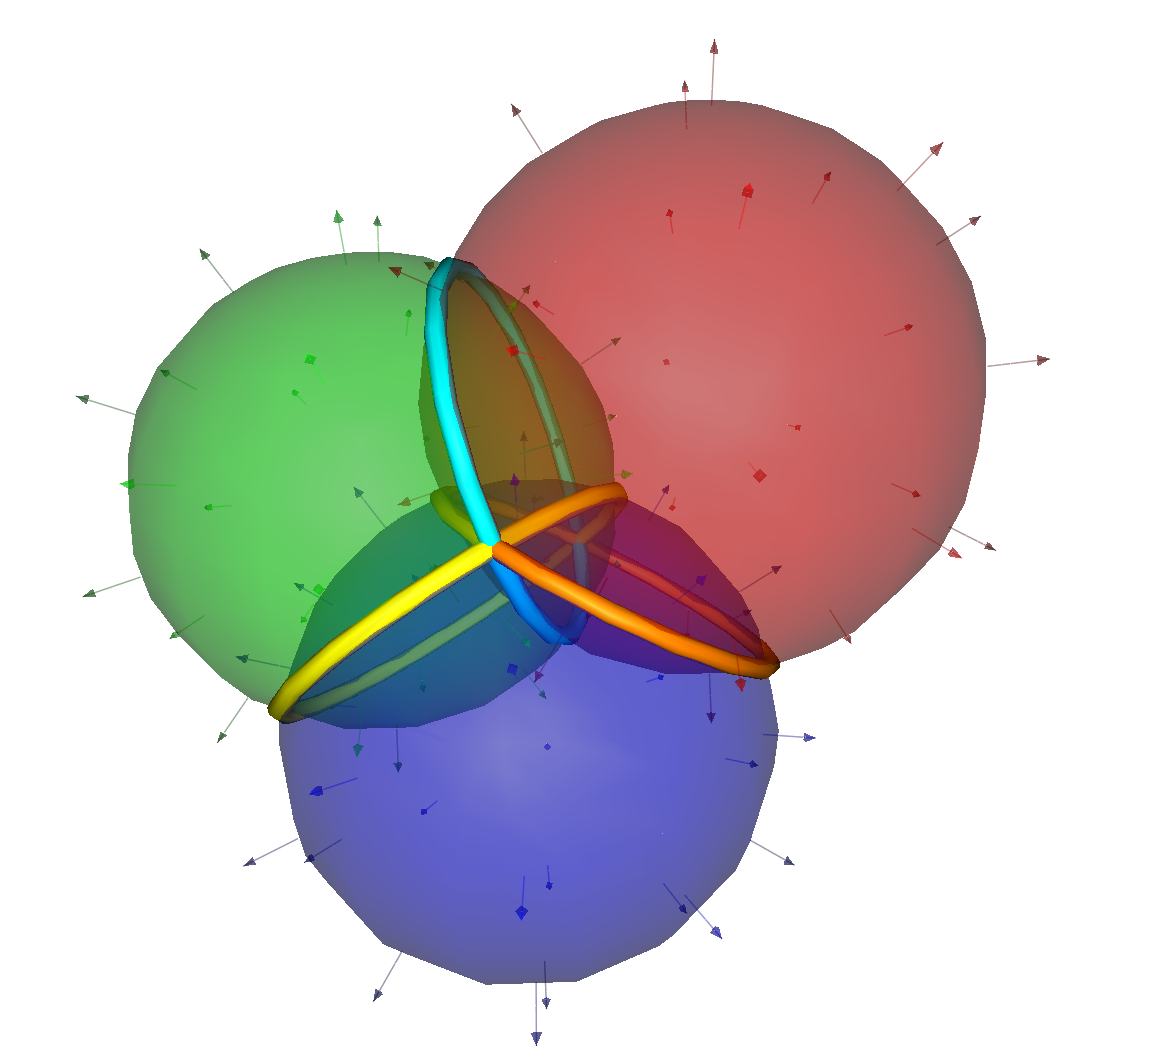
\includegraphics[scale=0.2]{Rounds}
\caption{3 Rounds, 3 Circles and 1 Point-Pair}
\end{figure}
\end{frame}

\begin{frame}
\frametitle{$(n-1)$-dimensional \alert{Dual} Hyper-Planes}
The function $p(x)$ factors out of the equation
\begin{equation*}
(x-c)\cdot v = 0
\end{equation*}
as the alternative equation
\begin{equation*}
p(x)\cdot\left(v+(c\cdot v)\nvai\right) = 0.
\end{equation*}
\end{frame}

\begin{frame}
\frametitle{Generating All \alert{Dual Flats} Of CGA}
Let $\{\pi_k\}_{k=1}^m$ be $m$ planes of dimension $n-1$ having a \alert{non-empty} and
\alert{non-degenerate} intersection.\pause

Then the blade $B$, given by
\begin{equation*}
B = \bigwedge_{k=1}^m\pi_k,
\end{equation*}
\alert{dually} represents an $(n-m)$-dimensional hyper-plane.\pause

\alert{Flats} at infinity are \alert{free blades}.\pause

$0$-dimensional \alert{flats} are called \alert{flat points}.
\end{frame}
%====================================
% By non degenerate, here we mean that no two planes are parallel, and therefore
% also not the same plane.
% We will ignore free blades here to keep things simple.
% Again, be sure to mention the connection between dimension and grade here.
% There is nothing more or less that characterizes a flat point from a round point.
%====================================

\begin{frame}
\frametitle{All Flats Of CGA For 3-dimensional Space}
\begin{figure}
\centering
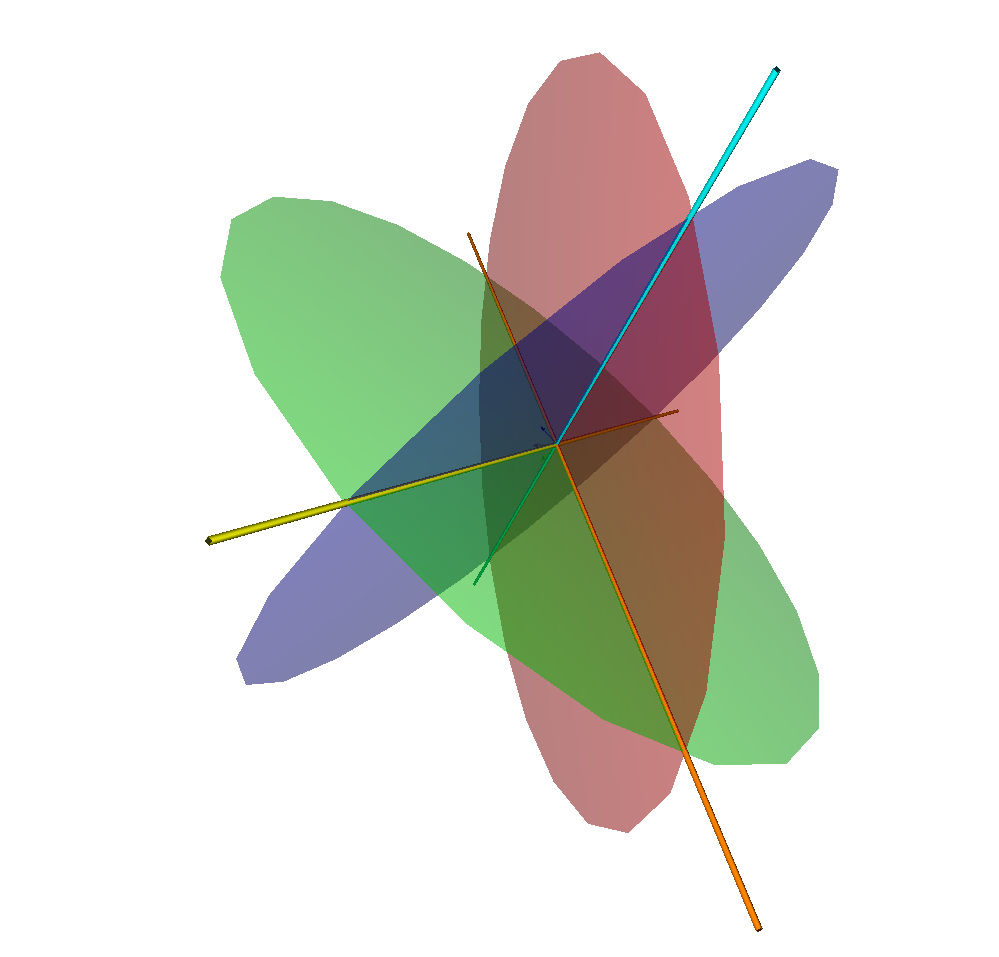
\includegraphics[scale=0.2]{Flats}
\caption{3 Planes, 3 Lines, 1 Flat-Point}
\end{figure}
\end{frame}
%====================================
% Flat points are going to be an exception in a few cases.
% Flat points play an interesting role in CGA, complementary to round points.
%====================================

\begin{frame}
\frametitle{A Generalization Of Coplanarity}
\begin{definition}
For $m\geq 0$, a set of points are \alert{co-$m$-hyper-planar} if...
\begin{equation*}
\begin{array}{l}
\mbox{For $m=0$, the points are identical,} \\
\mbox{For $m=1$, the points are collinear,} \\
\mbox{For $m=2$, the points are coplanar,} \\
\mbox{For $m=3$, the points are co-hyper-planar,} \\
\mbox{etc...}
\end{array}
\end{equation*}
\end{definition}
\end{frame}

\begin{frame}
\frametitle{A Condition For Linear Independents Of Points}
\begin{lemma}
For $m\geq 1$, if $m+1$ points $\{x_k\}_{k=1}^{m+1}\subset\V^n$ are non-co-$(m-1)$-hyper-planar,
then $\{p(x_k)\}_{k=1}^{m+1}$ is a linearly independent set.
\end{lemma}\pause
The proof is not hard, but too big for this slide.
\end{frame}

\begin{frame}
\frametitle{Generating All \alert{Direct Rounds} Of CGA}
Let $m\geq 1$.
For $m+1$ points $\{x_k\}_{k=1}^{m+1}\subset\V^n$ on an $m$-dimensional
hyper-sphere that are non-co-$(m-1)$-hyper-planar,
the blade $B$, given by
\begin{equation*}
B = \bigwedge_{k=1}^{m+1} p(x_k)
\end{equation*}
\alert{directly} represents the $m$-dimensional hyper-sphere.\pause
\begin{proof}
Let the $(n-m+1)$-blade $A$ \alert{dually} represent the $m$-dimensional hyper-sphere determined by the points.
If $A$ \alert{dually} represents this sphere, then $A^*$ \alert{directly} represents this sphere.
Therefore, we need to show that there exists $\lambda\in\R$ such that $A^*=\lambda B$.
For all $k$, we have $p(x_k)\in A^*$ and $p(x_k)\in B$.
By our lemma, $\{p(x_k)\}_{k=1}^m$ is a linearly independent set.
Lastly, $\grade(B) = m+1 = n+2-(n-m+1) = n+2-\grade(A) = \grade(A^*)$.
\end{proof}
\end{frame}
%====================================
% Be sure to emphasize that there is no difference between the two
% geometries that are a direct round and a dual round of the same dimension.
% The only difference is in how we're representing them.
% Be enthusiastic here!  This is a neat result!
%====================================

\begin{frame}
\frametitle{A Generalization Of Cospherical}
\begin{definition}
For $m\geq 1$, a set of points are \alert{co-$m$-hyper-spherical} if...
\begin{equation*}
\begin{array}{l}
\mbox{For $m=1$, the points are co-point-pair,} \\
\mbox{For $m=2$, the points are co-circular,} \\
\mbox{For $m=3$, the points are co-spherical,} \\
\mbox{For $m=4$, the points are co-hyper-spherical,} \\
\mbox{etc...}
\end{array}
\end{equation*}
\end{definition}
\end{frame}

\begin{frame}
\frametitle{Generating \alert{Almost} All \alert{Direct Flats} Of CGA}
Let $m\geq 1$.
For $m+2$ points $\{x_k\}_{k=1}^{m+2}\subset\V^n$ on an $m$-dimensional hyper-plane that
are \alert{(1)} non-co-$(m-1)$-hyper-planar and \alert{(2)} non-co-$m$-hyper-spherical, the blade $B$,
given by
\begin{equation*}
B = \bigwedge_{k=1}^{m+2} p(x_k),
\end{equation*}
\alert{directly} represents the $m$-dimensional hyper-plane.\pause
\begin{proof}
By \alert{(1)}, there exists the $(n-m)$-blade $A$ \alert{dually} representative of the
$m$-dimensional hyper-plane.  By \alert{(2)}, $B\neq 0$.  Lastly,
$\grade(B)=m+2=n+2-(n-m)=n+2-\grade(A)=\grade(A^*)$.
\end{proof}
\end{frame}
%====================================
% Condition 2 uses what we know about directly rounds!
% This argument does not work for direct flat points!
%====================================

\begin{frame}
\frametitle{Generating All \alert{Direct Flats} Of CGA}
Let $m\geq 0$.  For $m+1$ points $\{x_k\}_{k=1}^{m+1}\subset\V^n$ on an $m$-dimensional
hyepr-plane that are non-co-$(m-1)$-hyper-planar, the blade $B$, give by
\begin{equation*}
B = \nvai\wedge\bigwedge_{k=1}^{m+1} p(x_k),
\end{equation*}
\alert{directly} represents the $m$-dimensional hyper-plane.\pause

The proof, again, is not hard, but can't fit here.
\end{frame}
%====================================
%====================================

\begin{frame}
\frametitle{Quiz Time!}
\alert{Question}: Given a \alert{dual} line $L$ and a point $P$ not on $L$,
how do I find the \alert{dual} plane $N$ containing $L$ and $P$?\pause

\alert{Answer}: $N = (P\wedge L^*)^* = P\cdot L$.\pause

%\alert{Question}: Given a \alert{dual} circle $C$ and a point $P$ not on $C$ or on
%the plane determined by $C$, how do I find the \alert{dual} sphere $S$ containing $C$ and $P$?\pause
%
%\alert{Answer}: $S = (P\wedge C^*)^* = P\cdot C$.\pause

\alert{Question}: Let $S$ be a \alert{dual} sphere that intersects a \alert{dual} plane $N$ in more than one point, and let $P$ be a point on $S$ but not on $N$.  Then, if $P'$ is the reflection of $P$ about $N$, what is the \alert{dual} sphere reflection $S'$ of $S$ about $N$?\pause

\alert{Answer}: $S' = (P'\wedge(S\wedge N)^*)^* = P'\cdot(S\wedge N) = (P'\cdot S)N - (P'\cdot N)S$.
\end{frame}

\begin{frame}
\frametitle{The Fun Just Doesn't Stop!}
\alert{Question}: Let $S$ \alert{dually} represent the planet Saturn and let the $R$ \alert{directly} represent
one of Saturn's rings.  If this ring fell out of orbit, let the \alert{direct} circle $F$ on the surface of $S$ approximate
the debris field.  What is $F$?\pause

\alert{Answer}: $F = (S\wedge (R\wedge\nvai)^*)^* = S\cdot (R\wedge\nvai) = (S\cdot R)\nvai - (S\cdot\nvai)R$.\pause

\alert{Question}: Let $\{N_k\}_{k=0}^3$ be 4 \alert{dual} planes forming the sides of
a non-degenerate tetrahedron, and let $S$ be a \alert{dual} sphere containing all
4 vertices of the tetrahedron.  If all planes are known, how do we find $S$?
If $S$ is known and all planes save one, how do we find the remaining plane?\pause

\alert{Answer}: Not very pretty!

\end{frame}

\begin{frame}
\frametitle{Pictures Of Quiz Answers}
\begin{figure}
\centering
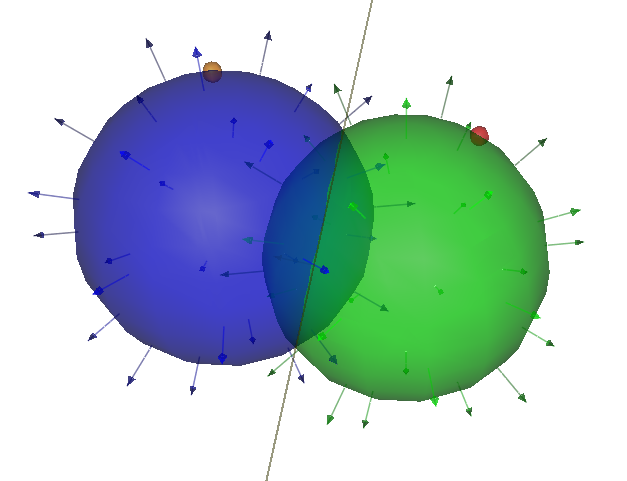
\includegraphics[scale=0.4]{SphereReflectionAboutPlane}
\caption{blah}
\end{figure}
\end{frame}

\begin{frame}
\frametitle{Pictures Of Quiz Answers (Continued)}
\begin{figure}
\centering
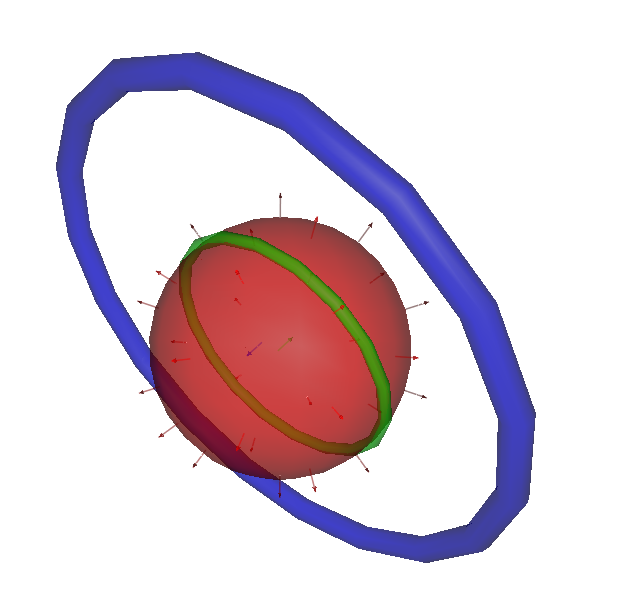
\includegraphics[scale=0.3]{FallenRingOfSaturn}
\caption{Saturn's Fallen Ring}
\end{figure}
\end{frame}

\begin{frame}
\frametitle{Transformations Of \alert{Direct} Geometry By Versors}
Recall the \alert{outermorphic} property of versors!\pause

Then, if the $m$-blade $B$ \alert{directly} represents
any geometry, (\alert{except a flat point}), then there exists $m$
points $\{x_k\}_{k=1}^m\subset\V^n$ such that
\begin{equation*}
VBV^{-1} = V\left(\bigwedge_{k=1}^m p(x_k)\right)V^{-1} = \bigwedge_{k=1}^m Vp(x_k)V^{-1}.
\end{equation*}\pause
Therefore, if we understand how $V$ transforms $p(x)$ for any $x\in\V^n$, then we can
predict how $V$ transforms any geometry, (\alert{except flat points})!\pause

If we know how a desired transformation transformas a point, then we have
found that transformation for any conformal geometry, (\alert{except flats points})!\pause

A versor may or may not leave $\nvai$ invariant under conjugation.
\end{frame}
%====================================
% As linear transformations are determined by how they
% transform a basis, versor transformations in CGA are
% determined by how they transform points!
%====================================

\begin{frame}
\frametitle{Transformations Of \alert{Dual} Geometry By Versors}
If the $m$-blade $B$ \alert{dually} represents any geometry, then we can write
\begin{equation*}
VBV^{-1} = V(B^*)^*V^{-1} = (VB^*V^{-1})^*,
\end{equation*}
relating this to what we know about the transformation of $\alert{directly}$ represented geometries.
\end{frame}
%====================================
%====================================

\begin{frame}
\frametitle{Types Of Transformations By Versors}
All conformal transformations can be represented by \alert{versors}!

Some of these include...
\begin{itemize}
\item \alert{Translations},
\item \alert{Rotations},
\item \alert{Dilations},
\item \alert{Transversions}.
\end{itemize}
\end{frame}
%====================================
% Here we see where the conformal model gets it's name.
% We can represent all conformal transformations by versors.
%====================================

\begin{frame}
\frametitle{Surprise!}
\alert{Blades} representative of geometry are also \alert{versors} representative of transformations!\pause
\begin{itemize}
\item \alert{Planar reflections} are represented by a dual planes!\pause
\item \alert{Spherical reflections} are represented by dual spheres!\pause
\item \alert{Translations} \& \alert{Rotations} are two successive planar reflections in well chosen planes.\pause
\item \alert{Dilations} \& \alert{Transversions} are two successive spherical reflections in well chosen spheres.\pause
\end{itemize}
\alert{Corollary}: We can use versors to transform transformations!\pause

\alert{Note}: Points are null, (non-invertible), and therefore, planar and spherical reflections \alert{generate} the versor group of all transformations.
\end{frame}
%====================================
% Here's another place to be enthusiastic!
% We can do reflections about hyper-planes of any dimension.
% We can do reflections about hyper-spheres of any dimension.
% Transforming a transform allows us to study a transformation
% as occurring at the origin without loss of generality.
%====================================

\begin{frame}
\frametitle{Planar Reflections}
\begin{figure}
\centering
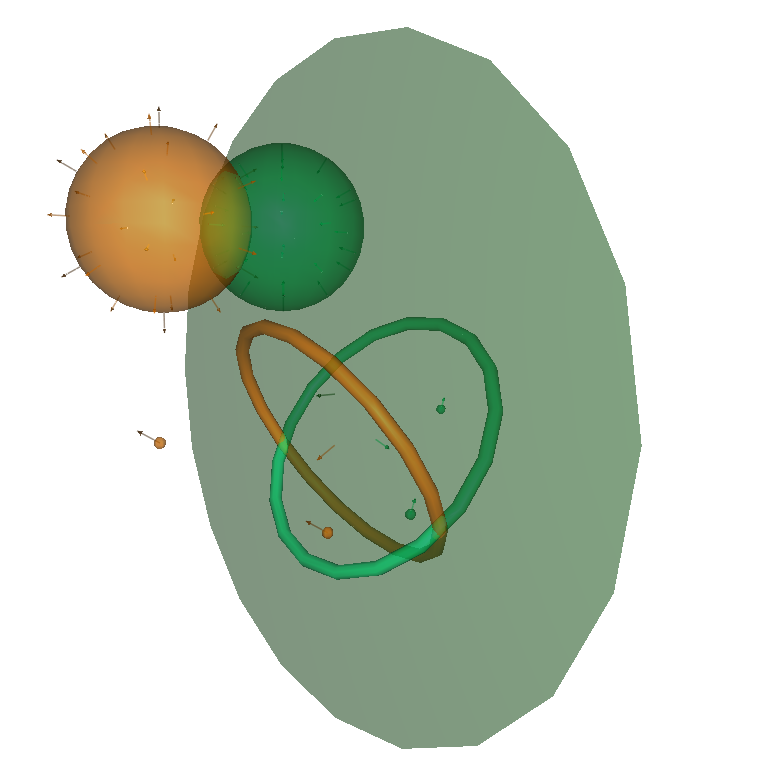
\includegraphics[scale=0.3]{PlanarReflectionsPerspectiveOne}
\caption{Planar reflections of a sphere, circle and point-pair.}
\end{figure}
\end{frame}

\begin{frame}
\frametitle{Planar Reflections (Again)}
\begin{figure}
\centering
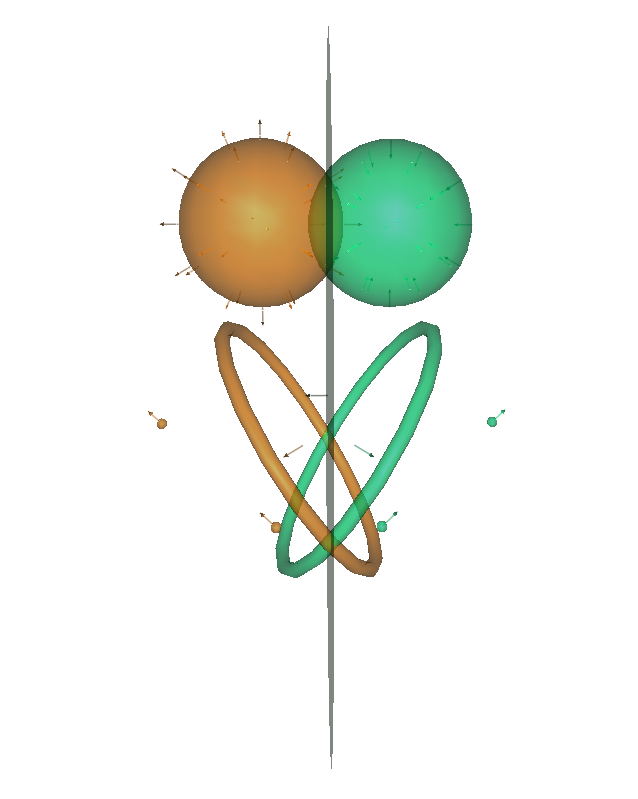
\includegraphics[scale=0.3]{PlanarReflectionsPerspectiveTwo}
\caption{Planar reflections of a sphere, circle and point-pair.}
\end{figure}
\end{frame}

\begin{frame}
\frametitle{Spherical Reflections}
\begin{figure}
\centering
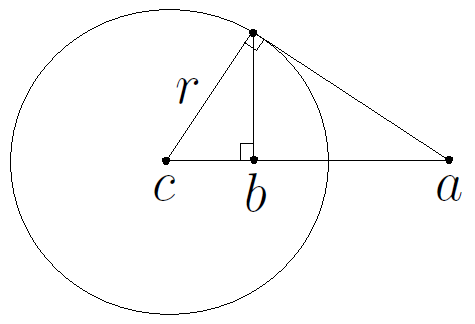
\includegraphics[scale=0.3]{SphericalReflectionFigure}
\caption{How we define spherical reflections.}
\end{figure}\pause
It can be shown that $b = c+\lambda(b-a)$, where $\lambda=r^2/(c-a)^2$.
\end{frame}

\begin{frame}
\frametitle{Spherical Reflections (Again)}
\begin{figure}
\centering
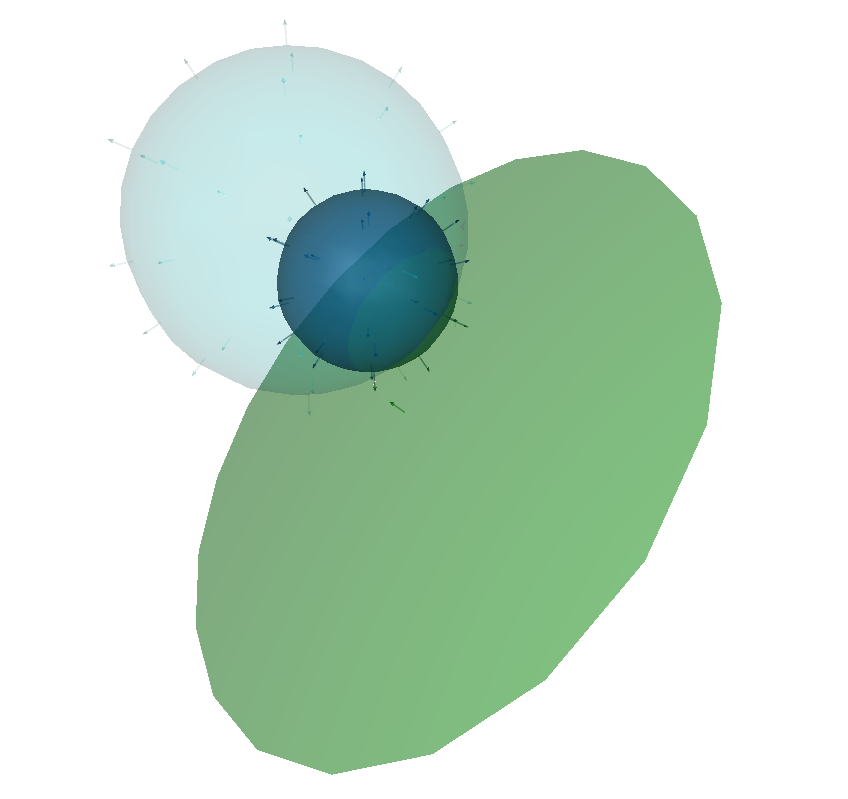
\includegraphics[scale=0.3]{SphericalReflectionPerspectiveOne}
\caption{The spherical reflection of a plane about a sphere is a sphere.}
\end{figure}
\end{frame}

\begin{frame}
\frametitle{Spherical Reflections (Yet Again)}
\begin{figure}
\centering
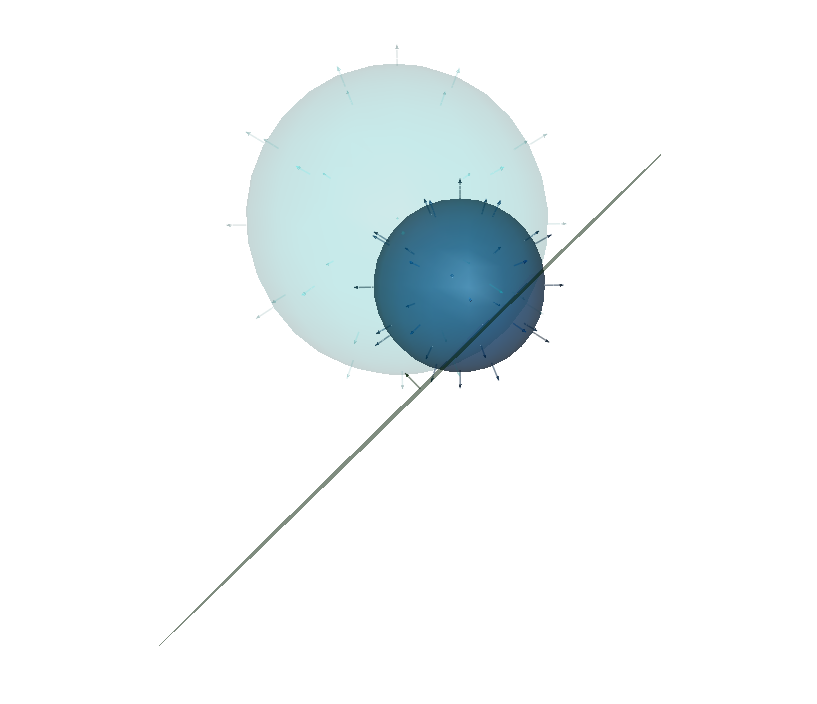
\includegraphics[scale=0.3]{SphericalReflectionPerspectiveTwo}
\caption{The spherical reflection of a plane about a sphere is a sphere.}
\end{figure}
\end{frame}

\begin{frame}
\frametitle{Rigid Body Motions}
\begin{figure}
\centering
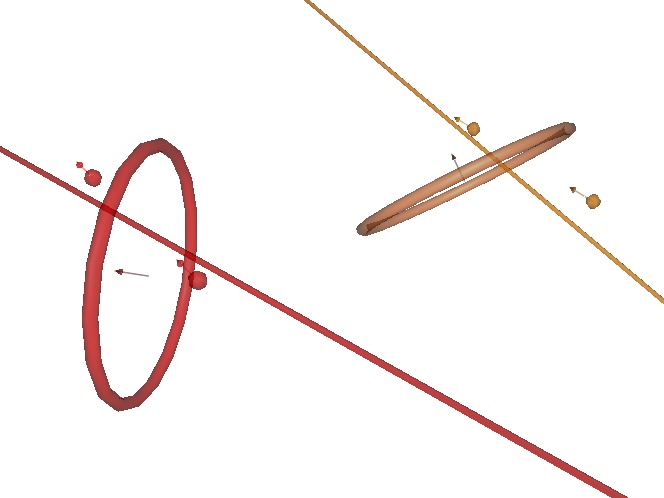
\includegraphics[scale=0.4]{TranslateRotatePerspectiveOne}
\caption{A line, circle and point-pair rotated/translated.}
\end{figure}
\end{frame}

\begin{frame}
\frametitle{Rigid Body Motions (Again)}
\begin{figure}
\centering
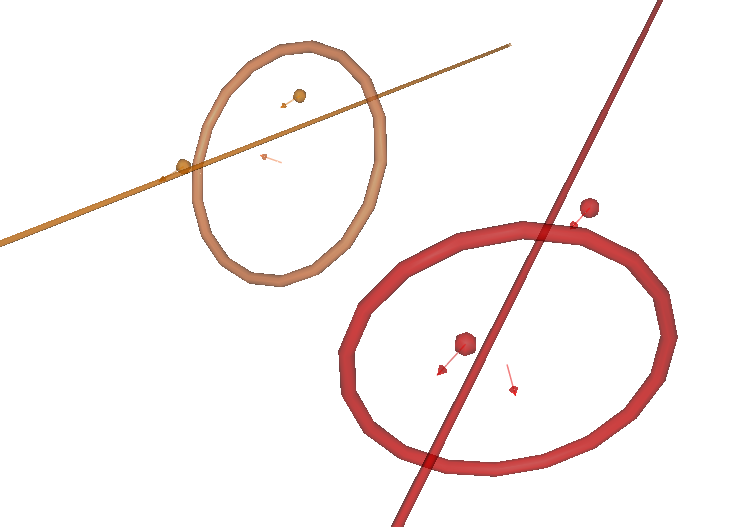
\includegraphics[scale=0.4]{TranslateRotatePerspectiveTwo}
\caption{A line, circle and point-pair rotated/translated.}
\end{figure}
\end{frame}

\begin{frame}
\frametitle{Dilations}
\begin{figure}
\centering
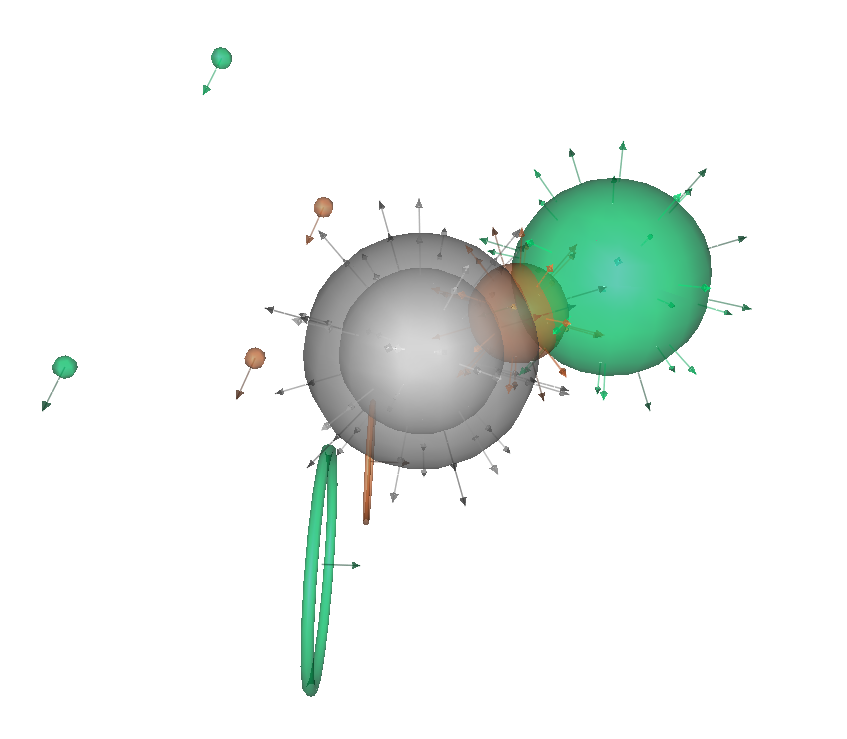
\includegraphics[scale=0.4]{DilationsPerspectiveOne}
\caption{Dilations of a circle, sphere and point-pair.}
\end{figure}
\end{frame}

\begin{frame}
\frametitle{Dilations (Again)}
\begin{figure}
\centering
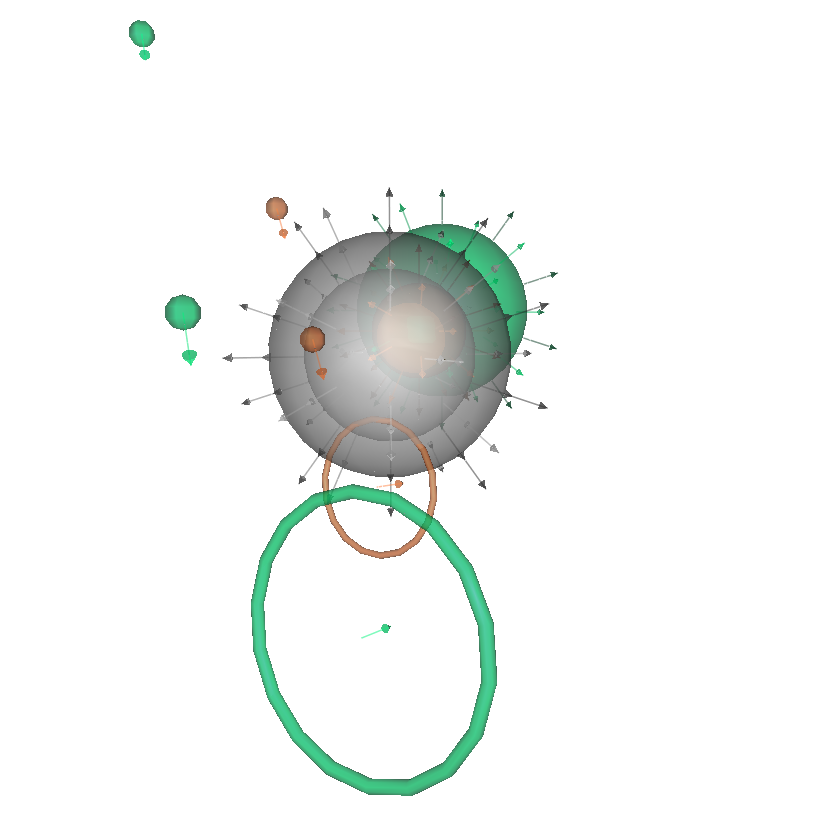
\includegraphics[scale=0.4]{DilationsPerspectiveTwo}
\caption{Dilations of a circle, sphere and point-pair.}
\end{figure}
\end{frame}

\begin{frame}
\frametitle{Transversions}
\begin{figure}
\centering
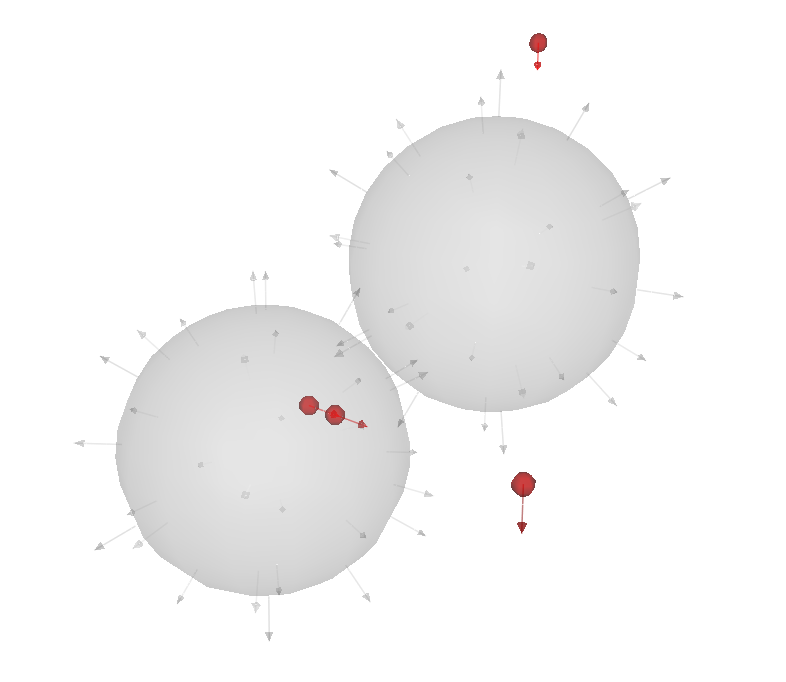
\includegraphics[scale=0.4]{TransversionOne}
\caption{The transversion of a point-pair.}
\end{figure}
\end{frame}

\begin{frame}
\frametitle{Transversions (Again)}
\begin{figure}
\centering
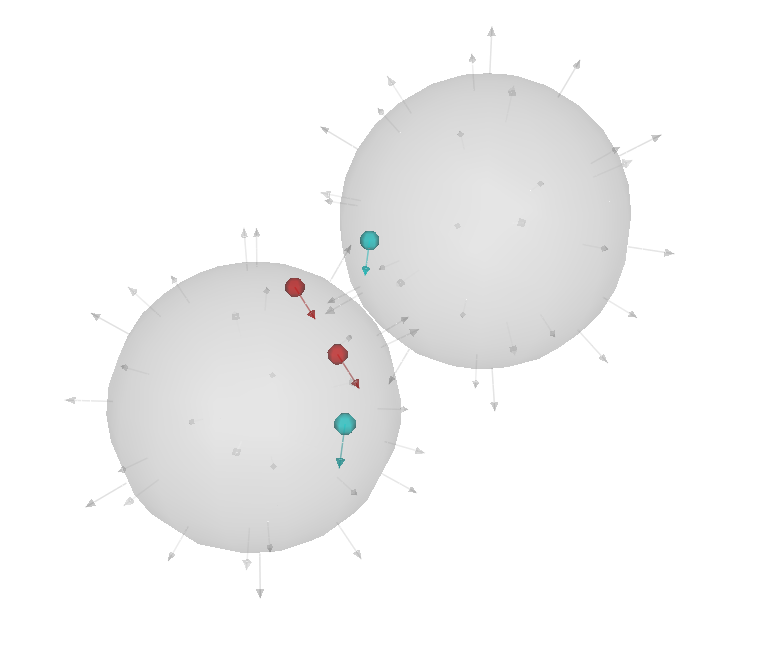
\includegraphics[scale=0.4]{TransversionTwo}
\caption{The transversion of some other point-pair.}
\end{figure}
\end{frame}

\begin{frame}
\frametitle{The End}
Thank you for your time.
Any questions?
\end{frame}

% do planar and spherical reflections
% show that planar and spherical reflections can be generalized to all lower dimensional prims

% We can build geos out of round-points using the outer product.
% We can build geos out of flat-points using...? versors transforms?

% limitations of CGA:
% -- not all quadratic forms supported

\end{document}